


\chapter{Introduction}
\section{Question de recherche}

A partir de données sur le climat, la qualité du sol et les pratiques culturales, est-il possible d’expliquer et de prédire les différents traits de la qualité en bouche des cafés du département de Risaralda ?



\section{Problématique}
Le sujet de ce Travail de Bachelor a été proposé par le « \textit{Centro Internacional de Agricultura Tropical }» (CIAT) qui travaille dans le but d’améliorer la productivité et la gestion de l’agriculture en zone tropicale, et dont les bureaux se trouvent à Cali, en Colombie.\\

À 200 kilomètres de Cali, le comité des caféiculteurs du département de Risaralda, une des région de l'Axe du Café \cite{EJE}, souhaite pouvoir expliquer les différents traits de la qualité en bouche des cafés produits dans les différents secteurs de leur département. La filière café colombienne est en effet en concurrence avec d’autres pays exportateurs sur le marché international, et un des avantages comparatifs de la Colombie est que ses terroirs produisent des cafés de qualité et de caractères affirmés. Il est donc stratégique pour la fédération des caféiculteurs de Colombie d'être en mesure de faire valoir ces spécificités pour aller chercher la valeur ajoutée associée aux produits démarqués du lot.


Ce projet a pour but de trouver des méthodes de modélisation afin d’identifier les caractéristiques du café spécifiques à chaque secteur de la région en se basant sur des analyses gustatives, des données climatiques et géographiques, et d’autres données de pratiques culturales.


Dans un premier temps, l’objectif est de catégoriser les cafés en tentant de trouver des tendances gustatives par rapport aux conditions de culture. Dans un second temps, il faudra pouvoir prédire la qualité en bouche des cafés par rapport aux conditions environnementales.


Le but de cette collaboration sur le long terme est de permettre au département de Risaralda de mettre en valeur la diversité de ses cafés, principalement à des fins de promotion auprès des acheteurs. 

\newpage
\section{Extraction des Données}
\paragraph{Les données gustatives}sont très relatives aux sens et à la perception de chaque goutteur. Cependant, la SCAA, \textit{Speciality Coffee Association of America}, dispose d’un système de notation basé sur des hypothèses communautaires reconnues ce qui permet d’avoir une certaine régularité dans les données de dégustations. Les cafés sont notés sur 100 points répartis sur plusieurs critères: parfum/arôme, saveur, arrière-goût, acidité, corps, équilibre, douceur, clean-cup (absence de défauts marqués), uniformité et évaluation personnelle du testeur.  Chacun de ces critères est noté sur 10 mais aussi par des termes qualitatifs. Par exemple, la saveur, c’est-à-dire la combinaison de l’odeur et du goût, la première impression qu’on a en goûtant le café, peut être notée 7/10 et “Caramel”. \\

Le premier échantillon de données reçu contenait toutes ces informations de manière uniforme mais il s'est avéré que la partie mandante n'avait pas pu uniformiser les données brutes dans les délais. Ainsi, les données finalement reçues variaient beaucoup d'un document à l'autre, d'une part dans les données de dégustations présentes et dans le type de document mais aussi dans les méta-données permettant d'identifier précisément de quelle café il s'agissait. Il a donc fallut effectuer un tri et ne garder que la masse qu'il était possible d'utiliser. Les critères permettant de garder une dégustation ou non sont les suivants: Identification possible du café grâce au numéro SICA ou au numéro d'identité du caféiculteur, présence des défauts physiques du café, présence des caractéristiques gustatives de manière uniforme.\\

 

\paragraph{Les données climatiques}comprennent les températures maximales, minimales et moyennes, la variation de température pendant la journée (DTR) et les quantités de précipitations. Les moyennes de ces mesures ont été calculée pour chaque mois et extrapolées sur une grande partie du territoire (à partir de stations météorologiques), permettant ainsi d’accéder aux mesures selon l’emplacement désiré à environ 500 mètres près. \\

En prenant par exemple les données de température maximale pour le mois de janvier 2011, en affectant pour chaque valeur une couleur, nous pouvons visualiser les données sous la forme d'une image comme sur la figure \ref{tmax_picture}.\\

Les données climatiques sont données de 2011 à 2016. il faudra cependant faire attention au fait qu'un café dégusté en février 2011 a poussé bien plus tôt. Les processus de récolte, de nettoyage, de fermentation, de séchage et de torréfaction du grain prennent du temps. Ce temps devra être pris en compte afin de sélectionner les bonnes données. 


\begin{figure}[H]
	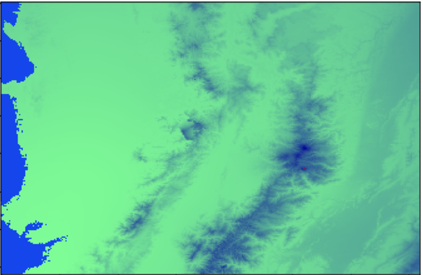
\includegraphics[scale=1]{tmax_picture_1}
	\caption{\label{tmax_picture} Mise sous forme graphique du tableau des température maximales pour le mois de janvier 2011 }
\end{figure}

\paragraph{Les données de qualité de sol}sont subdivisées en profils. Chaque profil est séparé en une ou plusieurs couches d’une certaine profondeur dont sont renseignées les caractéristiques comme le pH, la gravimétrie ou encore le taux de matière organique. Les données proviennent d'un GIS (Geographical Information System), d'où il est possible de croiser les données point par point afin d'extraire le profil de sol correspondant à un set de coordonnées GPS. 

%TODO
\paragraph{Le système SICA}, pour \textit{Sistema de Información Cafetera}, est un système géré par la Fédération Nationale des Caféiculteurs (FNC), permettant d'identifier chaque parcelle de production de café en Colombie\cite{SICA}. Il est important car c'est ce numéro qui permet, via les services de la FNC, d'avoir un identifiant unique pour chaque parcelle et d'y associer des informations la concernant.  


\chapter{Méthodes de modélisation}
\section{Rappel des objectifs}\label{obj}
Ce projet a deux principaux objectifs. Le premier est de trouver s'il existe différents groupes de café ayant des relations entre les conditions de culture et les caractéristiques physiques ou sensorielles. On cherche donc dans cette première partie à caractériser les cafés. On peut ici parler de clustering.  Le second objectif serait de prédire les caractéristiques physiques ou sensorielles à partir des données sur les conditions de culture. Nous avons donc ici plusieurs possibilités de manières d'agir. Par exemple, si le clustering a réussi à diviser les cafés en différentes classes, on cherchera à prédire dans quelle classe se situe un nouveau café. Plus spécifiquement, on pourra se concentrer sur certains attributs du café, par exemple l'acidité, afin d'estimer quelle sera la note attribuée. 



\newpage

\section{Apprentissage supervisé}
% knn, réseaux de neurones etc
Le but de l'apprentissage supervisé est d'expliquer des sorties (outputs) à partir d'entrées (inputs). Des règles sont calculées à partir de données d'apprentissage selon différents modèles. Par la suite, le modèle est utilisé pour catégoriser des nouvelles données. On essayera ici d'expliquer les données gustatives du café ou ses défauts physiques à l'aide des données climatiques et de sols. 


\subsection{Random Forest}

La méthode Random Forest, ou \textit{forêts d'arbres décisionnels} en français, fait partie des méthodes ensemblistes\cite{EnsembleMethods}, qui utilisent la combinaison de plusieurs modèles de base, d'apprentissage automatique. Elle combine les concepts de sous-espaces aléatoires et de bagging.\\

Le bagging\label{bagging}, ou \textit{bootstrap agregation}, consiste à sous-échantillonner (ou ré-échantillonner au hasard avec doublons) le set d'entrainement et de faire générer à l’algorithme voulu un modèle pour chaque sous-échantillon. On utilise le bagging pour réduire la variance de la fonction de prédiction estimée. Le bagging semble bien fonctionner pour les procédures avec une grande variance et un petit biais, comme les arbres de décision. \cite{hastie_09_elements-of.statistical-learning}\\


Random Forest effectue donc un apprentissage sur de multiples arbres de décision entraînés sur des sous-ensembles de données légèrement différents \cite{Statistics01randomforests}.


\begin{figure}[H]
	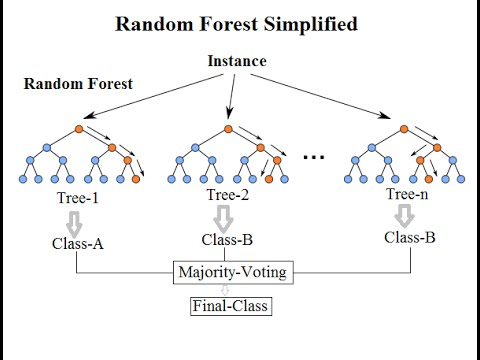
\includegraphics[scale=0.7]{RandomForestSimple}
	\caption{\label{RandomForestSchema} Schéma simple du fonctionnement de Random Forest. \newline Source: \textit{https://www.youtube.com/watch?v=ajTc5y3OqSQ}}
\end{figure}


\newpage

\section{Apprentissage non-supervisé}
Contrairement à l'apprentissage supervisé, l'apprentissage non-supervisé tente de trouver des groupes dans des données hétérogènes. Le but est d'extraire des connaissances à partir de ces données. Comme mentionné dans la partie \ref{obj}, notre but est de découvrir différents groupes de café identifiables. 


\subsection{SOM}

Les différentes classes gustatives d'un café peuvent être considérées comme des entrées afin vérifier s'il est possible de regrouper différents cafés qui se distingueraient. Afin de trouver les différentes catégories de café, nous testerons les capacités de l'algorithme SOM (pour Self Organizing Map ou Cartes Auto Adaptatives en français) qui utilise un réseau de neurones pour étudier la répartition des données dans un espace de grande dimension. 

Un bel exemple de SOM est celui de la carte de la pauvreté mondiale réalisé par le \textit{Department of Computer Science and Engineering} de l'université \textit{Helsinki University of Technology}. 

\begin{figure}[H]
	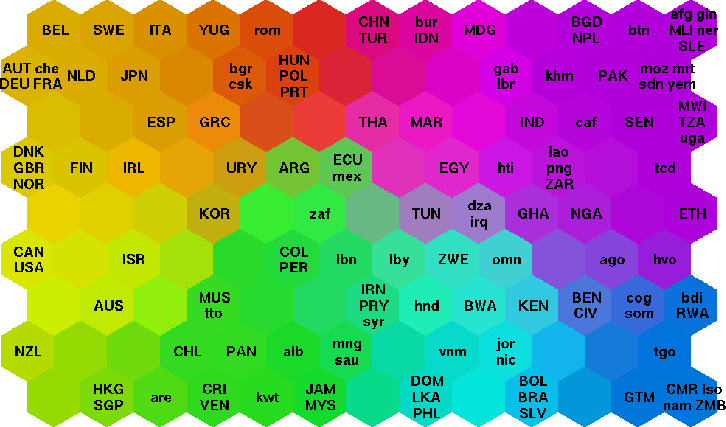
\includegraphics[scale=0.5]{SOMWordlPovertyMap}
	\caption{\label{SOMPovertyMap} Pays organisés en SOM d'après des indicateurs de pauvreté. \newline Source: \textit{http://www.cis.hut.fi/research/som-research/worldmap.html}}
\end{figure}

\begin{figure}[H]
	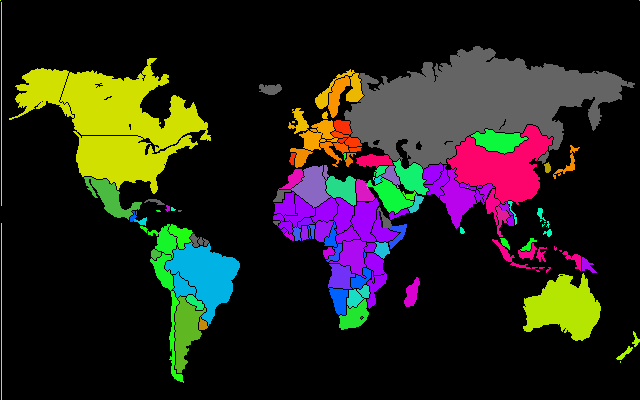
\includegraphics[scale=0.55]{worldmap}
	\caption{\label{WorldPovertyMap} Pays correspondants à la carte SOM de la figure \ref{SOMPovertyMap} \newline Source: \textit{http://www.cis.hut.fi/research/som-research/worldmap.html}}
\end{figure}




% TODO - clustering and association http://machinelearningmastery.com/supervised-and-unsupervised-machine-learning-algorithms/

\newpage
\section{Optimisation}

\subsection{Boosting}
Le principe du boosting est quelque peu différent du bagging (voir section \ref{bagging}). Les différents classifieurs sont pondérés de manière à ce qu’à chaque prédiction, les classificateurs ayant prédit correctement auront un poids plus fort que ceux dont la prédiction est incorrecte.\\


Adaboost est un algorithme de boosting qui s’appuie sur ce principe, avec un paramètre de mise à jour adaptatif permettant de donner plus d’importance aux valeurs difficiles à prédire, donc en boostant les classificateurs qui réussissent quand d’autres ont échoué. Des variantes permettent de l’étendre à la classification multiclasses. Adaboost s’appuie sur des classificateurs existants et cherche à leur affecter les bons poids vis à vis de leurs performances\cite{EnsembleMethods}.\\


\begin{figure}[H]
	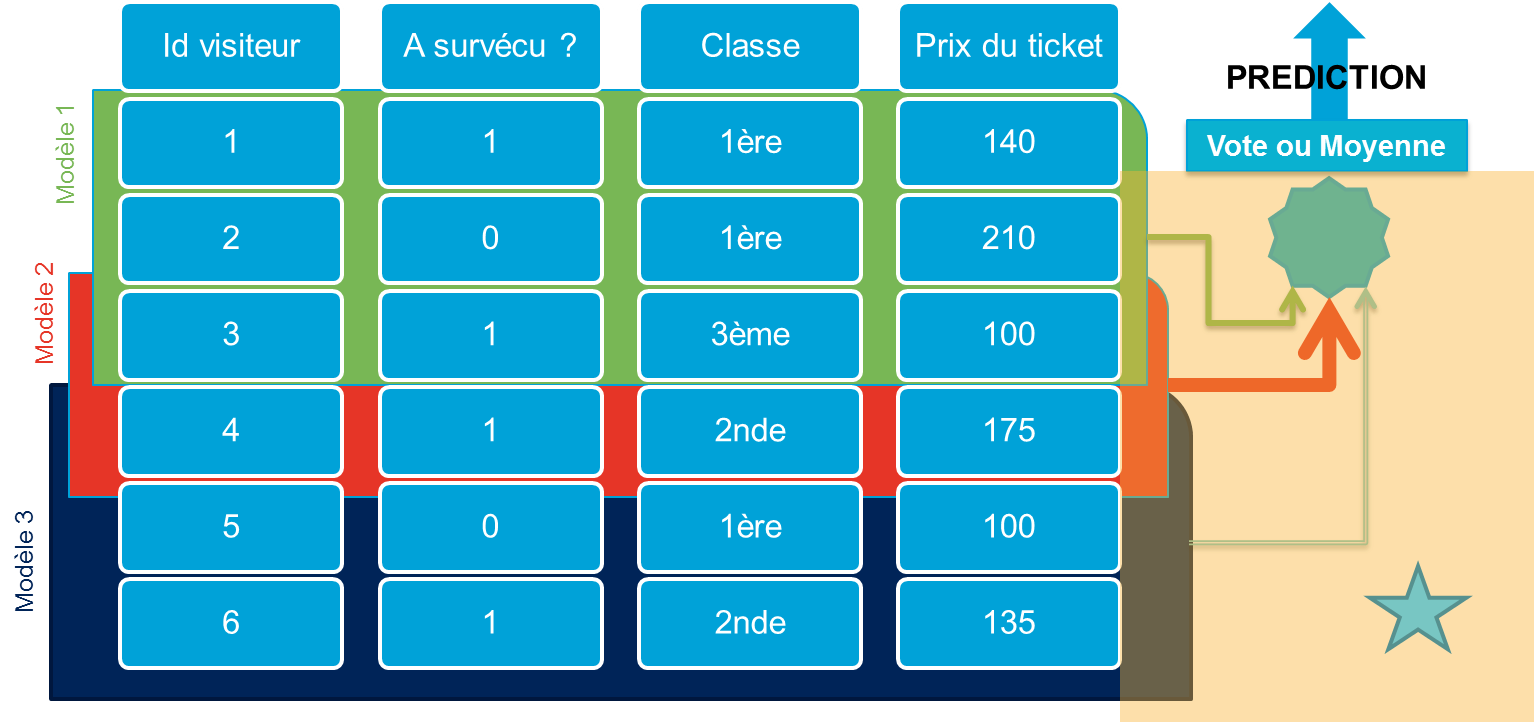
\includegraphics[scale=0.5]{boosting1}
	\caption{\label{BoostingSchema}Schéma du fonctionnement du Boosting \newline Source: \textit{http://www.cis.hut.fi/research/som-research/worldmap.html}}
\end{figure}

Gradient Boosting est une méthode de machine learning utilisée pour les problèmes de classification et de régression. Elle fait aussi partie des méthodes ensemblistes, et est utilisée majoritairement avec des arbres de décision. L'idées est encore d'agréger plusieurs classificateurs ensemble mais cette fois en les créant itérativement.\\


Le classifieur du gradient boosting est donc au final paramétré par les poids de pondération des différents mini-classifieurs, ainsi que par les paramètres des fonctions utilisées. Il s’agit donc d’explorer un espace de fonctions simples par une descente de gradient sur l’erreur\cite{EnsembleMethods}.

\subsection{Cross-Validation}

Contrairement au bagging qui est utilisé pour réduire l'overfitting en entrainant plusieurs modèles sur des données ré échantillonnées (avec répétition) puis en construisant un modèle sur la moyenne de ces modèles, la cross-validation est utilisée pour tester la fiabilité d'un modèle en se basant sur un échantillonnage des données d'entrainement et de test. Il existe plusieurs méthodes: « holdout method », « k-fold cross-validation » et « leave-one-out cross-validation ».\\

La première consiste à diviser le set de données en deux et en utilisant une partie pour entrainer le modèle puis une autre pour le tester. L'erreur est estimée en calculant un score de performance avec une méthode comme MSE (Erreur Quadratique Moyenne ou \textit{Mean Square Error}). \\

Étant donné que les données sont souvent trop peu nombreuses pour se permettre de laisser tomber dès le départ une partie des données, la k-fold cross-validation devient utile. On divise le set en k échantillons puis on en sélectionne un comme étant le set de test puis les k-1 autres comme étant le set d'entrainement. On répète l'opération en sélectionnant chaque fois un échantillon différent pour le test. Le score de performance est calculé en réalisant la moyenne des scores des k validations effectuées. La méthode « Leave-one out » utilise le même principe mais en ne laissant qu'une seule entrée en dehors du set d'entrainement à chaque tour\cite{hastie_09_elements-of.statistical-learning}. 


\chapter{Analyse préliminaire des données}


\section{Pre-processing}
Description du dataset (rapidement, le reste dans un codebook)\\

Mise en forme du dataset, une sortie à la fois vs plusieurs sorties etc \\
On considère les données gustatives et les défauts physiques comme des sorties -> les prendre un par un ou tous ensemble\\

Description du set, différentes parties des données, éventuelles données manquantes\\





\section{Data mining}
Extraction de features etc 
\subsection{Principal Component Analysis (PCA)}\label{PCAss}
La PCA, pour Analyse en Composantes Principales en français, est une méthode qui consiste à transformer un jeu de variables corrélées en nouvelles variables dé-corrélées les unes des autres. Ces nouvelles variables sont appelées composantes principales et permettent de rendre l'information moins redondante. Pour faire plus simple, l'utilité de la Composante Principale est de réduire le nombre de variables tout en gardant un maximum d'information. La figure \ref{PCAdefinition} montre une représentation graphique de la composante principale. 


\begin{figure}[H]
	\caption{\label{PCAdefinition} Description de l'Analyse en Composante Principale. (A) Description d'un objet simple de manière compliquée ( trois dimensions pour par exemple une ellipse en papier) (B) Trouver des nouvelles variables (axes de coordonnées) orthogonaux l'un à l'autre qui pointent dans les directions de la plus grande variance (C) Utiliser les nouvelles variables (axes) pour décrire l'objet d'une manière plus simple. }
	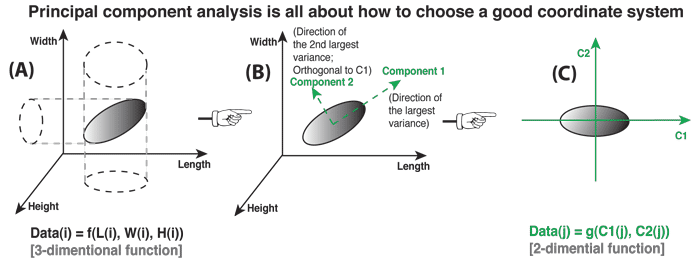
\includegraphics[scale=0.5]{PCA_1}
\end{figure}

On pourra ici éliminer les variables n'ayant pas une eigenvalue suffisamment importante afin de se concentrer sur les variables les plus importantes afin de réduire le nombre de dimension du dataset. 

\paragraph{Observation de la PCA pour les variables climatiques et de dégustations} Les différents types de variables, c'est-à-dire les données climatiques (températures, précipitations) ou les données de dégustations, on été réduits un par un sur 3 dimensions afin de pouvoir les visualiser sur un graphique et d'observer les différences entre les deux années disponibles. 

\begin{figure}[H]
	\caption{\label{PCAClimatAll} PCA sur les données climatiques (Tmin, Tmax, Tmean, DTR et Prec) }
	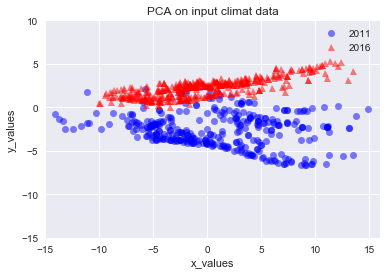
\includegraphics[scale=0.9]{PCA_Climat_All_1}
\end{figure}

% https://georgemdallas.wordpress.com/2013/10/30/principal-component-analysis-4-dummies-eigenvectors-eigenvalues-and-dimension-reduction/



